% Solutions for chapter 01-distributions
\providecommand{\oRC}[1]{{}^{1}\overline{#1}}       % one-point compactification
\providecommand{\qRC}[1]{{}^{q}\overline{#1}}       % quadratic compactification
\providecommand{\relRC}[2]{{}^{#1}\overline{#2}}    % compactification relative to a subspace

\section{Solutions for \cref{ch:distributions}: Tempered distributions and the Fourier transform}\label{solutions:distributions}

%----------------------------------------------------------------------
\subsection*{\Cref{distributions:ex:taylor}}
No. Idea: polynomial approximation at every point, with constants allowed to depend on
the point, controls $\phi$ but not the oscillation of its derivatives.

Let $\phi(x)=e^{-1/x^2}\sin(e^{1/x^2})$ for $x\neq0$ and $\phi(0)=0$.

\emph{The hypothesis holds.} At $\bar x\neq0$ the function $\phi$ is smooth on
$J=[\bar x-\frac12|\bar x|,\bar x+\frac12|\bar x|]$. Let $p_k(x;\bar x)$ be its Taylor
polynomial of degree $k$ at $\bar x$. Taylor's formula with Lagrange remainder gives
$|\phi(x)-p_k(x;\bar x)|\le C_k|x-\bar x|^{k+1}$ on $J$, with
$C_k=\sup_J|\phi^{(k+1)}|/(k+1)!$. So $\epsilon_k=\min(\frac12|\bar x|,C_k^{-1})$ works
(if $C_k=0$ take $\epsilon_k=\frac12|\bar x|$). At $\bar x=0$ take $p_k=0$. With
$y=x^{-2}$ we have $|\phi(x)|\,|x|^{-k-1}\le y^{(k+1)/2}e^{-y}\le M_k$, where
$M_k=\sup_{y>0}y^{(k+1)/2}e^{-y}<\infty$. Hence $|\phi(x)-0|\le M_k|x|^{k+1}$ for all $x$,
and $\epsilon_k=\min(1,M_k^{-1})$ works.

\emph{But $\phi$ is not $\mathcal{C}^1$.} It is differentiable everywhere: at $x\ne0$
clearly, and at $0$ with $\phi'(0)=0$ since $|\phi(x)|\le M_1x^2$. For $x\neq0$, since
$\frac d{dx}e^{\pm1/x^2}=\mp2x^{-3}e^{\pm1/x^2}$,
\[
  \phi'(x)=2x^{-3}e^{-1/x^2}\sin(e^{1/x^2})-2x^{-3}\cos(e^{1/x^2}).
\]
Let $x_m=(\log(2\pi m))^{-1/2}$, $m\in\N$. Then $e^{1/x_m^2}=2\pi m$, so the sine
vanishes, the cosine is $1$, and $\phi'(x_m)=-2x_m^{-3}\to-\infty$ as $x_m\downarrow0$.
So $\phi'$ is unbounded near $0$ and is not continuous at $0$; $\phi$ is not even
$\mathcal{C}^1$, let alone smooth.

What the hypothesis does give is weaker: with $k=1$ it says that $\phi$ is
differentiable at every point (the terms of degree $\ge2$ of $p_1$ are
$O(|x-\bar x|^2)$, so $p_1(\bar x)=\phi(\bar x)$ and the linear part of $p_1$ at $\bar x$
is the derivative). Smoothness would follow only with estimates that are locally
\emph{uniform} in $\bar x$; the example shows that pointwise estimates are not enough.

%----------------------------------------------------------------------
\subsection*{\Cref{distributions:ex:exp-cos}}
Idea: $u=v'$ with $v(x)=\sin(e^x)$ bounded, and $v'$ is defined by duality.

Let $v(x)=\sin(e^x)$; then $v\in\CI(\R)$, $|v|\le1$ and $v'(x)=e^x\cos(e^x)=u(x)$. Define
\[
  T(\phi)=-\int_\R\sin(e^x)\,\phi'(x)\,dx,\qquad\phi\in\cS(\R),
\]
that is, $T=\pa_xv=iDv$ in the sense of \eqref{distributions:eq:dual-ops}. It is
continuous:
$|T(\phi)|\le\int\ang{x}^{-2}dx\cdot\sup\ang{x}^2|\phi'|\le C\norm{\phi}_3$, so
$T\in\cSp(\R)$ by \cref{distributions:def:tempered}. If $\phi\in\CIc(\R)$, integration
by parts has no boundary terms and gives $\int u\phi\,dx=\int v'\phi\,dx=-\int v\phi'\,dx=T(\phi)$.

\emph{Uniqueness.} If $T'\in\cSp(\R)$ also satisfies $T'(\phi)=\int u\phi\,dx$ for
$\phi\in\CIc(\R)$, then $T-T'$ is continuous on $\cS(\R)$ and vanishes on $\CIc(\R)$,
which is dense by \cref{distributions:lem:cutoff}. Hence $T=T'$.

For every $\phi\in\cS(\R)$, $T(\phi)$ is the improper integral
$\lim_{R\to\infty}\int_{-R}^Ru\phi\,dx$: indeed
$\int_{-R}^Ru\phi=[v\phi]_{-R}^R-\int_{-R}^Rv\phi'$, and $v\phi(\pm R)\to0$.

\emph{The integral need not converge absolutely.} Let $\phi(x)=\exp(-\ang{x}^{1/2})$. Writing
$\phi=g(1+x^2)$ with $g(t)=\exp(-t^{1/4})$, each $g^{(j)}(t)$ is a finite sum of terms
$c\,t^{\gamma}\exp(-t^{1/4})$ with $\gamma\le0$, and by the chain rule $\phi^{(k)}$ is a
sum of products of $g^{(j)}(1+x^2)$ with polynomials in $x$. Hence
$|x^a\phi^{(k)}(x)|\le C\ang{x}^{M}\exp(-\ang{x}^{1/2})$ for some $M$, which is bounded,
so $\phi\in\cS(\R)$. Substituting $y=e^x$,
\[
  \int_0^\infty|u\phi|\,dx=\int_1^\infty|\cos y|\exp\big(-\ang{\log y}^{1/2}\big)\,dy.
\]
For $y\ge1$, $\ang{\log y}^{1/2}\le(1+\log y)^{1/2}\le\frac12\log y+1$ (since
$(1+t)^{1/2}\le1+t/2$), so the integrand is at least $e^{-1}y^{-1/2}|\cos y|$. On each
interval $[\pi j-\frac\pi3,\pi j+\frac\pi3]$, $j\ge1$, we have $|\cos y|\ge\frac12$, so the
integral is at least $\sum_j e^{-1}\frac\pi3\,(\pi j+\frac\pi3)^{-1/2}=\infty$.

%----------------------------------------------------------------------
\subsection*{\Cref{distributions:ex:metric}}
Let $f(t)=t/(1+t)=1-1/(1+t)$ for $t\ge0$. Then $f$ is increasing, $0\le f<1$, and $f$
is subadditive: for $a,b\ge0$,
\[
  f(a)+f(b)-f(a+b)=\frac a{1+a}-\frac a{1+a+b}+\frac b{1+b}-\frac b{1+a+b}\ge0.
\]
If $\norm{\cdot}$ is a norm, then $\norm{u+v}\le\norm u+\norm v$, so by monotonicity
and subadditivity $f(\norm{u+v})\le f(\norm u+\norm v)\le f(\norm u)+f(\norm v)$, which
is the hint.

Now $d(\phi,\psi)=\sum_k2^{-k}f(\norm{\phi-\psi}_k)$ converges, with $0\le d\le2$. It is
symmetric since $\norm{\psi-\phi}_k=\norm{\phi-\psi}_k$. If $d(\phi,\psi)=0$ then
$\norm{\phi-\psi}_0=\sup|\phi-\psi|=0$, so $\phi=\psi$; and $d(\phi,\phi)=0$. For the
triangle inequality apply the hint with $u=\phi-\chi$, $v=\chi-\psi$ to each norm
$\norm{\cdot}_k$, multiply by $2^{-k}$ and sum:
$d(\phi,\psi)\le d(\phi,\chi)+d(\chi,\psi)$. So $d$ is a metric.

%----------------------------------------------------------------------
\subsection*{\Cref{distributions:ex:cauchy}}
We treat Cauchy sequences; for convergence replace $\phi_l$ by $\phi$ throughout. Let
$f(t)=t/(1+t)$ as in the previous solution; $f$ is an increasing bijection
$[0,\infty)\to[0,1)$ with inverse $s\mapsto s/(1-s)$, and $f(t)\le t$.

Suppose $(\phi_j)$ is $d$-Cauchy and fix $k$. Since every term of the series is
non-negative, $f(\norm{\phi_j-\phi_l}_k)\le2^kd(\phi_j,\phi_l)$. Given $\epsilon>0$,
choose $J$ with $d(\phi_j,\phi_l)<2^{-k}\epsilon/(1+\epsilon)$ for $j,l\ge J$; then
$f(\norm{\phi_j-\phi_l}_k)<f(\epsilon)$, so $\norm{\phi_j-\phi_l}_k<\epsilon$.

Conversely, suppose $(\phi_j)$ is Cauchy for each $\norm{\cdot}_k$, and let $\epsilon>0$.
Choose $p$ with $2^{-p}<\epsilon/2$. By \eqref{distributions:eq:ball} (which uses
$f(t)\le t$, $f\le1$ and $\norm{\cdot}_k\le\norm{\cdot}_p$ for $k\le p$),
$d(\phi_j,\phi_l)\le2\norm{\phi_j-\phi_l}_p+2^{-p}$. Choose $J$ with
$\norm{\phi_j-\phi_l}_p<\epsilon/4$ for $j,l\ge J$. Then $d(\phi_j,\phi_l)<\epsilon$.

%----------------------------------------------------------------------
\subsection*{\Cref{distributions:ex:bilinear}}
Joint continuity refers to the product topology on $\cS(\R^n)\times\cS(\R^p)$, which is
given by the metric $d(\phi,\phi')+d(\psi,\psi')$.

Suppose $|B(\phi,\psi)|\le C\norm{\phi}_N\norm{\psi}_N$. If $\phi_j\to\phi$ and
$\psi_j\to\psi$, then $\norm{\psi_j}_N$ is bounded (\cref{distributions:ex:cauchy}) and
\begin{align*}
  |B(\phi_j,\psi_j)-B(\phi,\psi)|&\le|B(\phi_j-\phi,\psi_j)|+|B(\phi,\psi_j-\psi)|\\
  &\le C\norm{\phi_j-\phi}_N\norm{\psi_j}_N+C\norm{\phi}_N\norm{\psi_j-\psi}_N\to0.
\end{align*}
Since the spaces are metric, sequential continuity is continuity.

Conversely, let $B$ be continuous at $(0,0)$. There is $r>0$ such that $d(\phi,0)<r$ and
$d(\psi,0)<r$ imply $|B(\phi,\psi)|<1$. Choose $N$ with $2^{-N}<r/2$ and let
$\epsilon=r/4$. By \eqref{distributions:eq:ball}, $\norm{\phi}_N<\epsilon$ implies
$d(\phi,0)\le2\norm{\phi}_N+2^{-N}<r$, and likewise for $\psi$. Let $\phi,\psi\ne0$
(otherwise $B(\phi,\psi)=0$); then $\norm{\phi}_N,\norm{\psi}_N>0$ since these are norms.
For $0<t<\epsilon$, applying the above to $t\phi/\norm{\phi}_N$ and $t\psi/\norm{\psi}_N$
gives $t^2|B(\phi,\psi)|<\norm{\phi}_N\norm{\psi}_N$. Letting $t\uparrow\epsilon$,
$|B(\phi,\psi)|\le\epsilon^{-2}\norm{\phi}_N\norm{\psi}_N$.

Finally, if $B$ is only separately continuous, \cref{distributions:lem:joint} gives the
estimate with $N=p$, and the first part shows that $B$ is jointly continuous.

%----------------------------------------------------------------------
\subsection*{\Cref{distributions:ex:restriction}}
Write $x=(y,z)\in\R^k\times\R^{n-k}$, so $\pi_k^*f(y)=f(y,0)$. (For $k=0$ we read
$\cS(\R^0)=\C$ and $\pi_0^*f=f(0)$; for $k=n$ the map is the identity.)

\emph{Continuity.} For $\alpha,\beta\in\N_0^k$, differentiation in $y$ commutes with
setting $z=0$, so $y^\alpha D_y^\beta(\pi_k^*f)(y)=(x^{(\alpha,0)}D^{(\beta,0)}f)(y,0)$.
Taking suprema, $\norm{\pi_k^*f}_m\le\norm{f}_m$ for every $m$, so $\pi_k^*$ maps
$\cS(\R^n)$ into $\cS(\R^k)$ continuously by \cref{distributions:lem:continuity}.

\emph{Surjectivity.} Let $g\in\cS(\R^k)$ and $\rho(z)=e^{-|z|^2}\in\cS(\R^{n-k})$. Then
$f=g\boxtimes\rho\in\cS(\R^n)$ by the exterior product estimate of
\cref{distributions:sec:schwartz}, and $\pi_k^*f(y)=g(y)\rho(0)=g(y)$.

%----------------------------------------------------------------------
\subsection*{\Cref{distributions:ex:gaussian-contour}}
Idea: after completing the square the integrand is an entire function, and the
integral over a horizontal line does not depend on the line.

Let $n=1$ and $\xi\in\R$. Since
$-(x+\frac i2\xi)^2-\frac{\xi^2}4=-x^2-ix\xi$,
\[
  \int_\R e^{-ix\xi}e^{-x^2}dx=e^{-\xi^2/4}\int_\R h(x)\,dx,\qquad h(z)=e^{-(z+\frac i2\xi)^2}.
\]
The function $h$ is entire. Let $c=-\xi/2$ and let $\Gamma_R$ be the boundary of the
rectangle with vertices $-R$, $R$, $R+ic$, $-R+ic$, positively oriented if $c>0$
(if $c=0$ there is nothing to prove; if $c<0$ reverse orientation). By Cauchy's theorem
$\oint_{\Gamma_R}h\,dz=0$, that is
\[
  \int_{-R}^Rh(x)\,dx-\int_{-R}^Rh(x+ic)\,dx
  =-\int_0^{c}h(R+i\tau)\,i\,d\tau+\int_0^{c}h(-R+i\tau)\,i\,d\tau .
\]
For $z=\pm R+i\tau$ with $\tau$ between $0$ and $c$, we have $z+\frac i2\xi=\pm R+i\sigma$
with $|\sigma|\le|\xi|/2$, and $|e^{-(a+i\sigma)^2}|=e^{-a^2+\sigma^2}$. So each vertical
integral is bounded by $\frac{|\xi|}2e^{-R^2+\xi^2/4}\to0$ as $R\to\infty$. Since
$h(x+ic)=e^{-x^2}$ (the shift lands on $\operatorname{Im}x=-\xi/2$), letting $R\to\infty$
gives $\int_\R h(x)\,dx=\int_\R e^{-x^2}dx=\pi^{1/2}$. The last equality is the standard
Gaussian integral: $\big(\int e^{-x^2}dx\big)^2=\int_{\R^2}e^{-|x|^2}dx
=2\pi\int_0^\infty e^{-r^2}r\,dr=\pi$. Hence $\cF(e^{-x^2})(\xi)=\pi^{1/2}e^{-\xi^2/4}$.

For general $n$, $e^{-|x|^2}e^{-ix\cdot\xi}=\prod_je^{-x_j^2}e^{-ix_j\xi_j}$, so by Fubini
$\cF(e^{-|x|^2})(\xi)=\prod_j\pi^{1/2}e^{-\xi_j^2/4}=\pi^{n/2}e^{-|\xi|^2/4}$. The formula
for $\mathcal{G}$ follows exactly as in the proof of \cref{distributions:lem:gaussian},
by the substitution $\xi=2\eta$, which turns it into $(2\pi)^{-n}2^n\cF(e^{-|\eta|^2})(-2x)$.

%----------------------------------------------------------------------
\subsection*{\Cref{distributions:ex:L2}}
Let $\phi\in L^2(\R^n)$ and $\psi\in\cS(\R^n)$. By the Cauchy--Schwarz inequality,
$\phi\psi\in L^1$ and
\[
  |T_\phi(\psi)|\le\norm{\phi}_{L^2}\norm{\psi}_{L^2}
  \le\norm{\phi}_{L^2}\Big(\int\ang{x}^{-2n-2}dx\Big)^{1/2}\sup\ang{x}^{n+1}|\psi|
  \le C\norm{\phi}_{L^2}\norm{\psi}_{n+1}.
\]
($\ang{x}^{-2n-2}$ is integrable, being $O(|x|^{-2n-2})$ with $2n+2>n$.) So $T_\phi$ is
well defined, linear in $\psi$ and continuous, i.e.\ $T_\phi\in\cSp(\R^n)$, and
$\phi\mapsto T_\phi$ is linear.

\emph{Injectivity.} Suppose $T_\phi=0$. Since $\cS(\R^n)\supset\CIc(\R^n)$ is dense in
$L^2(\R^n)$ (the standard fact used in \cref{distributions:prop:plancherel}), there are
$\psi_j\in\cS(\R^n)$ with $\psi_j\to\bar\phi$ in $L^2$. By Cauchy--Schwarz
$0=T_\phi(\psi_j)=\int\phi\psi_j\,dx\to\int\phi\bar\phi\,dx=\norm{\phi}^2_{L^2}$, so
$\phi=0$ in $L^2$.

%----------------------------------------------------------------------
\subsection*{\Cref{distributions:ex:sobolev}}
(a) Let $Q(x)=\{t\in\R^n;\ t_j\le x_j\ \forall j\}$, so $v(x)=\int\mathbf 1_{Q(x)}f\,dt$.
Then $|v(x)|\le\norm{f}_{L^1}$. If $y\to x$ then $\mathbf 1_{Q(y)}(t)\to\mathbf 1_{Q(x)}(t)$
for every $t$ outside the null set $\bigcup_j\{t_j=x_j\}$, and $|\mathbf 1_{Q(y)}f|\le|f|$;
by dominated convergence $v(y)\to v(x)$. So $v$ is bounded and continuous, and in
particular $v\in\cSp(\R^n)$; also $f\in\cSp(\R^n)$ since $|\int f\psi|\le\norm{f}_{L^1}\norm{\psi}_0$.

Let $\psi\in\cS(\R^n)$. Since $D_j^t=-D_j$ and $D_j=-i\pa_j$,
\[
  (D_1\cdots D_nv)(\psi)=v\big((-D_1)\cdots(-D_n)\psi\big)
  =(-1)^n(-i)^n\int v(x)\,\pa_1\cdots\pa_n\psi(x)\,dx.
\]
The function $(t,x)\mapsto\mathbf 1_{Q(x)}(t)f(t)\,\pa_1\cdots\pa_n\psi(x)$ is integrable
on $\R^{2n}$, so by Fubini
\[
  \int v\,\pa_1\cdots\pa_n\psi\,dx=\int f(t)\Big(\int_{t_1}^\infty\!\!\cdots\int_{t_n}^\infty
  \pa_1\cdots\pa_n\psi(x)\,dx_n\cdots dx_1\Big)dt=(-1)^n\int f\psi\,dt,
\]
because each $\int_{t_j}^\infty\pa_jg\,dx_j=-g|_{x_j=t_j}$ for $g$ rapidly decreasing.
Hence $(D_1\cdots D_nv)(\psi)=(-1)^n(-i)^n(-1)^n\int f\psi=(-i)^n\int f\psi$, i.e.\
$D_1\cdots D_nv=(-i)^nf$.

For the inclusion: if $g\in L^2$ then by Cauchy--Schwarz
$\int(1+|x|)^{-n-1}|g|\,dx\le\norm{(1+|x|)^{-n-1}}_{L^2}\norm{g}_{L^2}$, and
$\int(1+|x|)^{-2n-2}dx=|\Sphere^{n-1}|\int_0^\infty r^{n-1}(1+r)^{-2n-2}dr<\infty$.

(b) The hypothesis means that $\hat u$ is a function of the form
$\hat u=\ang{\xi}^{-s}h$ with $h\in L^2(\R^n)$ (multiplication by $\ang{\xi}^{-s}\in\CIb$
is defined on $\cSp$, and this is the meaning of $\ang\xi^s\hat u\in L^2$). Put
$g=\ang{\xi}^{-s}h$. For $|\alpha|\le k$, $|\xi^\alpha g|\le\ang{\xi}^{k-s}|h|$ by
\eqref{distributions:eq:japanese}, and $\ang{\xi}^{k-s}\in L^2$ because $2(s-k)>n$.
By Cauchy--Schwarz, $\xi^\alpha g\in L^1$ for all $|\alpha|\le k$. Define
\[
  w(x)=\int e^{ix\cdot\xi}g(\xi)\,\dbar\xi .
\]
Since $g\in L^1$, $w$ is bounded and continuous (dominated convergence). Since
$|D_x^\alpha e^{ix\cdot\xi}g|=|\xi^\alpha g|$ is integrable and independent of $x$ for
$|\alpha|\le k$, the theorem on differentiation under the integral sign, applied $k$ times,
shows $w\in\mathcal{C}^k$ with $D^\alpha w(x)=\int e^{ix\cdot\xi}\xi^\alpha g\,\dbar\xi$,
which is again bounded and continuous.

It remains to see $u=w$. By \cref{distributions:cor:FT-dist}, $u=\mathcal{G}\hat u$, so
for $\phi\in\cS(\R^n)$, using Fubini ($g\in L^1$, $\phi\in L^1$),
\[
  u(\phi)=\hat u(\mathcal{G}\phi)=\int g(\xi)\int e^{ix\cdot\xi}\phi(x)\,dx\,\dbar\xi
  =\int w(x)\phi(x)\,dx .
\]
Thus $u=w\in\mathcal{C}^k(\R^n)$. Finally the distributional derivatives $D^\alpha u$,
$|\alpha|\le k$, equal the classical ones, because integration by parts against
$\phi\in\cS$ has no boundary terms ($D^\beta w$ bounded, $\phi$ rapidly decreasing). So
$D^\alpha u$ is bounded and continuous for $|\alpha|\le k$.

%----------------------------------------------------------------------
\subsection*{\Cref{distributions:ex:support}}
Let $\phi$ be continuous with $|\phi|\le C\ang{x}^N$; then $\ang{x}^{-N-n-1}\phi\in L^1$
and $T_\phi\in\cSp(\R^n)$. Let $F=\overline{\{x;\ \phi(x)\neq0\}}$.

$\supp T_\phi\subset F$: the open set $O=\R^n\setminus F$ satisfies $\phi=0$ on $O$, so
$T_\phi(\psi)=\int\phi\psi=0$ for $\psi\in\CIc(O)$. Thus $T_\phi$ vanishes on $O$ and
$\supp T_\phi\subset F$.

$F\subset\supp T_\phi$: since $\supp T_\phi$ is closed, it suffices to show that
$\phi(x_0)\neq0$ implies $x_0\in\supp T_\phi$, i.e.\ that $T_\phi$ does not vanish on any
open $O\ni x_0$. Replacing $\phi$ by $i\phi$ if necessary, $\operatorname{Re}\phi(x_0)\neq0$,
say $>0$ (else replace $\phi$ by $-\phi$). By continuity $\operatorname{Re}\phi>0$ on a
ball $B(x_0,r)\subset O$. Let $\psi(x)=\exp(-1/(r^2-|x-x_0|^2))$ for $|x-x_0|<r$ and
$\psi=0$ otherwise; then $\psi\in\CIc(O)$, $\psi\ge0$, $\psi>0$ on $B(x_0,r)$. Hence
$\operatorname{Re}T_\phi(\psi)=\int\operatorname{Re}\phi\,\psi\,dx>0$, so $T_\phi$ does not vanish on $O$.

For $\delta$: if $\psi\in\CIc(\R^n\setminus\{0\})$ then $\delta(\psi)=\psi(0)=0$, so
$\supp\delta\subset\{0\}$. If $O\ni0$ is open, a bump $\psi\in\CIc(O)$ with $\psi(0)=1$
(as above) gives $\delta(\psi)\ne0$; so $0\in\supp\delta$ and $\supp\delta=\{0\}$.

%----------------------------------------------------------------------
\subsection*{\Cref{distributions:ex:peetre}}
\emph{Locality.} Let $P=\sum_{|\alpha|\le m}p_\alpha(x)D^\alpha$ with $p_\alpha\in\CIb$.
By \eqref{distributions:eq:dual-ops}, for $u\in\cSp$ and $\psi\in\cS$,
\[
  (Pu)(\psi)=u(P^t\psi),\qquad P^t\psi=\sum_{|\alpha|\le m}(-D)^\alpha(p_\alpha\psi).
\]
Let $O=\R^n\setminus\supp u$, on which $u$ vanishes. If $\psi\in\CIc(O)$, then
$P^t\psi$ is smooth and $\supp P^t\psi\subset\supp\psi$, a compact subset of $O$, so
$P^t\psi\in\CIc(O)$ and $(Pu)(\psi)=0$. Thus $Pu$ vanishes on $O$, i.e.\
$\supp Pu\subset\supp u$.

\emph{Peetre's theorem: the continuous case in full.} Suppose in addition that
$P\colon\cS(\R^n)\to\cS(\R^n)$ is continuous, local and $\supp Pu\subset K$ for all $u$.
We show $P$ is a differential operator with coefficients in $\CIc(\R^n)\subset\CIb(\R^n)$.

By \cref{distributions:lem:continuity}, $\sup|Pu|=\norm{Pu}_0\le C\norm{u}_N$ for some
$C,N$. For $x_0\in\R^n$ let $\ell_{x_0}(u)=(Pu)(x_0)$; so $\ell_{x_0}\in\cSp$ with
$|\ell_{x_0}(u)|\le C\norm{u}_N$. Its support is in $\{x_0\}$: if
$u\in\CIc(\R^n\setminus\{x_0\})$ then $x_0$ has a neighbourhood $O$ disjoint from
$\supp u\supset\supp Pu$; so the continuous function $Pu$ vanishes on $O$ and
$\ell_{x_0}(u)=0$. Let $\tau u(x)=u(x+x_0)$; then $\tau$ and $\tau^{-1}$ are continuous
on $\cS$ with $\norm{\tau^{-1}u}_N\le C_{x_0}\norm{u}_N$ (expand $(x-x_0)^\alpha$), so
$\ell_{x_0}\circ\tau^{-1}$ has support in $\{0\}$ and order $N$. The proof of
\cref{distributions:thm:point-support} (with $k=N$) gives
\[
  (Pu)(x_0)=\sum_{|\alpha|\le N}a_\alpha(x_0)\,\pa^\alpha u(x_0),\qquad u\in\cS(\R^n),
\]
with $N$ independent of $x_0$. The coefficients are unique, since the functionals
$u\mapsto\pa^\alpha u(x_0)$ are linearly independent (test on $\chi(x)(x-x_0)^\beta$,
$\chi=1$ near $x_0$). For $x_0\notin K$, $\ell_{x_0}=0$, so $a_\alpha(x_0)=0$.

\emph{The coefficients are smooth.} Fix $R$ and $\chi\in\CIc(\R^n)$ with $\chi=1$ on
$\{|x|<R\}$, and let $u_\beta=\chi x^\beta/\beta!$. For $|x|<R$,
$Pu_\beta(x)=\sum_{\alpha\le\beta}a_\alpha(x)x^{\beta-\alpha}/(\beta-\alpha)!$. For
$\beta=0$ this says $a_0=P(\chi)$ is smooth on $\{|x|<R\}$; by induction on $|\beta|$,
$a_\beta=Pu_\beta-\sum_{\alpha<\beta}a_\alpha x^{\beta-\alpha}/(\beta-\alpha)!$ is smooth there.
As $R$ is arbitrary, $a_\alpha\in\CI$, and $\supp a_\alpha\subset K$. Hence
$P=\sum_{|\alpha|\le N}a_\alpha\pa^\alpha$, a differential operator with
$\CIc$ coefficients.

\emph{Without continuity (sketch, as requested).} Peetre's theorem does not assume
continuity, and the work lies in proving an a priori bound on the order. The key lemma
is: for each $x_0$ there are a neighbourhood $U$ and $C,k$ with
$\sup|Pu|\le C\sum_{|\alpha|\le k}\sup|\pa^\alpha u|$ for all $u\in\CIc(U\setminus\{x_0\})$.
If it failed, one could choose $u_j$ supported in disjoint balls shrinking to $x_0$, with
$\sum_{|\alpha|\le j}\sup|\pa^\alpha u_j|\le2^{-j}$ but $\sup|Pu_j|\ge j$ (normalize a
violating function). Then $u=\sum u_j$ is smooth (for fixed $\alpha$ the series of
$\pa^\alpha u_j$ converges uniformly), and by locality $Pu=Pu_j$ near $\supp u_j$, so
$Pu$ would be unbounded near $x_0$, contradicting $Pu\in\cS$. Covering $K$ by finitely
many such $U$, the lemma together with locality and
\cref{distributions:thm:point-support} (applied to $u\mapsto Pu(x)$, $x\neq x_0$) shows
that $P$ is a differential operator of bounded order away from finitely many points;
a second application of the same argument at those points gives a global order, and the
smoothness of the coefficients follows as above.

%----------------------------------------------------------------------
\subsection*{\Cref{distributions:ex:delta-rep}}
Let $w=\frac12e^{-|x|}$, bounded and continuous. For $\phi\in\cS(\R)$, since $D^t=-D$,
$(1+D^2)w(\phi)=w((1+D^2)\phi)=\frac12\int e^{-|x|}(\phi-\phi'')\,dx$. Integrating by parts
twice on each half line,
\begin{align*}
  \int_0^\infty e^{-x}\phi''\,dx&=-\phi'(0)+\int_0^\infty e^{-x}\phi'\,dx
  =-\phi'(0)-\phi(0)+\int_0^\infty e^{-x}\phi\,dx,\\
  \int_{-\infty}^0e^{x}\phi''\,dx&=\phi'(0)-\int_{-\infty}^0e^{x}\phi'\,dx
  =\phi'(0)-\phi(0)+\int_{-\infty}^0e^{x}\phi\,dx.
\end{align*}
Adding, $\int e^{-|x|}\phi''=-2\phi(0)+\int e^{-|x|}\phi$, so
$(1+D^2)w(\phi)=\phi(0)$, i.e.\ $\delta=(1+D^2)w$. (Equivalently,
$\hat w=(1+\xi^2)^{-1}$ and $\hat\delta=1$, by \eqref{distributions:eq:PD}.)

\emph{$\delta=Dw$ with $w$ bounded and continuous is impossible.} Let $H$ be the
Heaviside function. For $\phi\in\cS(\R)$, $(DH)(\phi)=-H(D\phi)=i\int_0^\infty\phi'=-i\phi(0)$,
so $D(iH)=\delta$. If $Dw=\delta$, then $D(w-iH)=0$, so by \cref{distributions:lem:Dju}
(with $n=1$, where $\cSp(\R^0)=\C$ and $1\boxtimes c$ is the constant $c$) $w-iH=c$ is a
constant. So $w=iH+c$ almost everywhere. A continuous function equal almost everywhere
to $c$ on $(-\infty,0)$ equals $c$ there, hence $w(0)=c$; likewise $w=c+i$ on
$(0,\infty)$, so $w(0)=c+i$: a contradiction. Thus $\delta$ is the derivative of a
bounded function ($iH$) but not of a bounded continuous one.

%----------------------------------------------------------------------
\subsection*{\Cref{distributions:ex:exterior}}
Define $A\colon\cS(\R^m)\to\cSp(\R^n)$ by $A\psi=v(\psi)\,u$. It is linear, and it is
continuous for the weak topology: for each $\phi$, $\psi\mapsto(A\psi)(\phi)=u(\phi)v(\psi)$
is continuous because $v$ is. By \cref{distributions:thm:kernel} there is
$K\in\cSp(\R^{n+m})$ with $K(\phi\boxtimes\psi)=(A\psi)(\phi)=u(\phi)v(\psi)$; set
$u\boxtimes v=K$. If $K'$ is another such distribution, then $K-K'$ is continuous and
vanishes on finite sums of exterior products, which are dense by
\cref{distributions:lem:tensor-dense}; so $K=K'$.

%----------------------------------------------------------------------
\subsection*{\Cref{distributions:ex:conformal}}
\emph{Definition.} A \emph{conformal structure} on a real vector space $W$ of dimension
$n$ is an equivalence class $[g]$ of inner products on $W$, where $g\sim g'$ if
$g'=cg$ for some constant $c>0$. A linear map $G\colon(W,[g])\to(W',[g'])$ is
\emph{conformal} if $G^*g'\in[g]$. A \emph{conformal frame} is a linear isomorphism
$L\colon W\to\R^n$ that is an isometry from $(W,g)$ to Euclidean $\R^n$ for some $g\in[g]$.

\emph{The compactification.} Recall from \cref{distributions:sec:one-point} that
$\oRC{\R^n}=\Sphere^n$ has the charts $z=2Z/(1+Z_0)$ on $\Sphere^n\setminus\{\text{south pole}\}$
and $w=2Z/(1-Z_0)$ on $\Sphere^n\setminus\{\text{north pole}\}$, related by $w=\iota(z)=4z/|z|^2$
(indeed $|z|^2=4(1-Z_0)/(1+Z_0)$, so $4z/|z|^2=2Z/(1-Z_0)$), with $\infty$ at $w=0$.
For $(W,[g])$ set $\oRC{W}=W\sqcup\{\infty\}$, and give it the smooth structure that
makes $\tilde L\colon\oRC W\to\oRC{\R^n}$, $\tilde L|_W=L$, $\tilde L(\infty)=\infty$, a
diffeomorphism, for a conformal frame $L$. If $L'$ is another conformal frame, with
$|L'w|^2=g'(w,w)$ and $g'=cg$, then $G=L'L^{-1}\in\GL(n,\R)$ satisfies
$|Gx|^2=c|x|^2$, so $G=c^{1/2}O$ with $O\in\mathrm{O}(n)$. In the chart $w$ near
$\infty$, $G$ becomes $h(w)=\iota(G\iota(w))=c^{-1/2}Ow$ (proof of
\cref{distributions:prop:one-point}, using $\iota\circ\iota=\Id$), and in the chart $z$ it
is linear. So $\tilde G=\tilde L'\tilde L^{-1}$ is smooth, as is its inverse (the same for
$G^{-1}=c^{-1/2}O^{-1}$). Hence the two smooth structures coincide: $\oRC W$ depends only
on $[g]$. (It does depend on $[g]$: by \cref{distributions:prop:one-point}, if
$[g]\neq[g']$ the identity of $W$ is not even $\mathcal{C}^1$ as a map between the two
compactifications, since $L'L^{-1}$ is then not conformal.)

\emph{Subspaces.} Let $V\subset W$ have dimension $k$ and carry the induced class
$[g|_V]$. Choose $g\in[g]$ and a $g$-orthonormal basis of $W$ whose first $k$ vectors lie
in $V$. The corresponding frame $L$ maps $V$ onto $\R^k\times\{0\}$, and $L|_V$ is a
conformal frame of $V$. So it suffices to treat $j\colon\R^k\ni z'\mapsto(z',0)\in\R^n$,
extended by $\infty\mapsto\infty$. In the chart $z$ it is linear. In the charts $w$ near
$\infty$, $\iota_n(z',0)=(4z'/|z'|^2,0)=(\iota_k(z'),0)$, so $j$ becomes $w'\mapsto(w',0)$,
including $w'=0\mapsto0$. Hence $j$ extends to a smooth map $\oRC V\to\oRC W$; it is an
injective immersion of a compact manifold, hence an embedding.

%----------------------------------------------------------------------
\subsection*{\Cref{distributions:ex:qrc-abstract}}
Let $W$ have dimension $n$ and $\mathbb{S}W=(W\setminus0)/\R^+$. For a linear isomorphism
$L\colon W\to\R^n$ define the bijection
\[
  Q_L\colon W\sqcup\mathbb{S}W\to\mathbb{B}^n,\qquad
  Q_L(w)=\frac{Lw}{\ang{Lw}},\qquad Q_L([w])=\frac{Lw}{|Lw|}.
\]
It is a bijection: $\mathrm{Q}$ maps $\R^n$ onto the open ball
(\eqref{distributions:eq:QRC}), and $[w]\mapsto Lw/|Lw|$ is well defined and bijective
from rays in $W$ to $\Sphere^{n-1}$. Define $\qRC W$ as the set $W\sqcup\mathbb{S}W$ with the
smooth structure making $Q_L$ a diffeomorphism onto $\mathbb{B}^n=\qRC{\R^n}$.

\emph{Independence of $L$.} For another $L'$ let $G=L'L^{-1}$. On the open ball,
$Q_{L'}Q_L^{-1}(y)=\mathrm{Q}(G\mathrm{Q}^{-1}y)=Gy/(1-|y|^2+|Gy|^2)^{1/2}$ by the
proof of \cref{distributions:prop:QRC}(ii). At $|y|=1$, $y=Lw/|Lw|$ is sent to
$L'w/|L'w|=Gy/|Gy|$, which is the same formula since $1-|y|^2=0$. So
$Q_{L'}Q_L^{-1}$ is the diffeomorphism of \cref{distributions:prop:QRC}(ii) on all of
$\mathbb{B}^n$, and the two smooth structures agree.

\emph{Same set, different structure.} By \cref{distributions:rem:RC-set} and
\cref{distributions:prop:affine}, $\RC W$ is also $W\sqcup\mathbb{S}W$, with $[w]$
corresponding (in a frame $L$) to the boundary point $(0,Lw/|Lw|)$ of $\Sphere^n_+$. In
the frames the identity of $W\sqcup\mathbb{S}W$ becomes the projection
$\pi\colon\Sphere^n_+\to\mathbb{B}^n$, $X\mapsto X'$: indeed
$\pi(\mathrm{RC}(z))=z/\ang z=\mathrm{Q}(z)$ and $\pi(0,\omega)=\omega$. Thus
$\Id\colon\RC W\to\qRC W$ is a smooth homeomorphism (a continuous bijection of compact
Hausdorff spaces). Its inverse $y\mapsto((1-|y|^2)^{1/2},y)$ is not smooth: the function
$\ang z^{-1}=(1-|y|^2)^{1/2}$, which is smooth on $\RC W$, has
$\frac{d}{dt}(1-t^2)^{1/2}=-t(1-t^2)^{-1/2}\to-\infty$ along $y=t\omega$, $t\uparrow1$.
So the topologies agree but the smooth structures differ.

%----------------------------------------------------------------------
\subsection*{\Cref{distributions:ex:projection}}
\emph{Correction.} As originally stated (``a linear map \dots\ extends continuously if
and only if it is injective'') the claim is false: the zero map $V\to W$, $\dim V>0$, is
not injective but extends to the constant map $\RC V\to\{\mathrm{RC}(0)\}\subset\RC W$,
which is smooth. The statement has been corrected to non-zero maps; we prove that
version. (So: a linear map extends continuously if and only if it is injective or zero.)

\emph{The projection.} Let $\pi(z_1,z_2)=z_1$. For $c\in\R$ and $t\to\infty$,
$\mathrm{RC}(c,t)=(1,c,t)/\ang{(c,t)}\to(0,0,1)$, the same boundary point for all $c$,
while $\mathrm{RC}(\pi(c,t))=(1,c)/\ang c$ is constant in $t$. A continuous extension
$F$ would satisfy $F(0,0,1)=(1,c)/\ang c$ for every $c$, which is impossible since these
values differ for different $c$.

\emph{General case.} Let $A\colon V\to W$ be linear, $\dim V,\dim W>0$, $A\neq0$. Fix
inner products and identify $V,W$ with Euclidean spaces (\cref{distributions:prop:affine}
and \cref{distributions:ex:qrc-abstract} show this is harmless). If $A$ is injective it
is an isomorphism onto $A(V)$ followed by the inclusion $A(V)\subset W$. The
isomorphism extends to a diffeomorphism of radial (\cref{distributions:prop:affine}) and
quadratic (\cref{distributions:prop:QRC}(ii)) compactifications, and the inclusion
extends smoothly by \cref{distributions:prop:inclusion}. So $A$ extends, even smoothly.

If $A$ is not injective, pick $0\ne e\in\ker A$ and $c\in V$ with $Ac\neq0$. For
$b\in\{0,c\}$ and $t\to\infty$, $b+te\to$ the boundary point $(0,e/|e|)$ of $\RC V$, since
$(1,b+te)/\ang{b+te}\to(0,e/|e|)$; likewise $\mathrm{Q}(b+te)\to e/|e|$ in $\qRC V$. But
$A(b+te)=Ab$ is constant in $t$. A continuous extension $F$ would therefore give
$F(\text{point})=\mathrm{RC}(0)$ and $=\mathrm{RC}(Ac)$, which differ because
$\mathrm{RC}$ (or $\mathrm{Q}$) is injective on $W$. Hence $A$ does not extend
continuously.

%----------------------------------------------------------------------
\subsection*{\Cref{distributions:ex:trivial}}
Recall $\RC{\{0\}}=\Sphere^0_+=\{X_0\in\R;\ X_0\ge0,\ |X_0|=1\}=\{1\}$ is a point, with
$\mathrm{RC}_{\{0\}}(0)=1$, and $\ang0=1$.

$V=\{0\}$: then $U=W$ and \eqref{distributions:eq:relRC} reads
$R_V(0,u)=(\mathrm{RC}_W(u),\mathrm{RC}_{\{0\}}(0))=(\mathrm{RC}_W(u),1)$. Thus
$\relRC{\{0\}}W=\RC W\times\{1\}$, and the identification is $\mathrm{RC}_W$. In the
explicit formulae, $s=1$ and $v'$ is absent.

$V=W$: then $U=\{0\}$, $\ang u=1$, and $R_V(v,0)=(1,\mathrm{RC}_W(v))$, so
$\relRC WW=\{1\}\times\RC W$ with identification $\mathrm{RC}_W$; here $t=1$, $u'$ is
absent, $s=\ang v^{-1}$ and $v'=v/\ang v$.

In both cases the only choice is a metric on $W$, and by \cref{distributions:prop:affine}
the smooth structure of $\RC W$ does not depend on it. So both are canonically $\RC W$.

%----------------------------------------------------------------------
\subsection*{\Cref{distributions:ex:doubly}}
Idea: all seven components are smooth functions of $\mathrm{RC}_V(v)$, $\mathrm{RC}_U(u)$
and the ``angle'' $(\ang u,\ang v)/|(\ang u,\ang v)|$; this triple lives on an explicit
manifold with corners $M$, the blow-up of the corner of $\RC V\times\RC U$.
(Its identification with both iterated blow-ups is \cref{blowup:prop:doubly}.)

Let $k=\dim V\ge1$, $l=\dim U\ge1$ (if one of them is $0$ everything reduces to
\cref{distributions:ex:trivial}), and identify $V=\R^k$, $U=\R^l$ isometrically. Write
\[
  X=(X_0,X')=\mathrm{RC}_V(v)\in\Sphere^k_+,\quad Y=(Y_0,Y')=\mathrm{RC}_U(u)\in\Sphere^l_+,\quad
  (a,b)=\frac{(\ang u,\ang v)}{(\ang u^2+\ang v^2)^{1/2}}.
\]
Then $a,b>0$, $a^2+b^2=1$ and $a/b=\ang u/\ang v=X_0/Y_0$, i.e.\ $aY_0=bX_0$.

\emph{The model.} Let $\mathcal{Q}=\{(a,b);\ a,b\ge0,\ a^2+b^2=1\}$ and
\[
  M=\{(X,Y,a,b)\in\Sphere^k_+\times\Sphere^l_+\times\mathcal{Q};\ aY_0=bX_0\},
\]
a compact subset of $\R^{k+1}\times\R^{l+1}\times\R^2$. We check that $M$ is a manifold
with corners by exhibiting charts which are restrictions of smooth maps, with smooth
inverses.
\begin{itemize}
\item $M_1=M\cap\{(X_0,Y_0)\neq(0,0)\}$. Here $aY_0=bX_0$ forces $(a,b)$ to be parallel
  to $(X_0,Y_0)$, and both lie in the closed first quadrant, so
  $(a,b)=(X_0,Y_0)/|(X_0,Y_0)|$. The projection $(X,Y,a,b)\mapsto(X,Y)$ is a bijection of
  $M_1$ onto the open subset $\Sphere^k_+\times\Sphere^l_+\setminus(\{X_0=0\}\times\{Y_0=0\})$
  of a product of manifolds with boundary, with smooth inverse
  $(X,Y)\mapsto(X,Y,(X_0,Y_0)/|(X_0,Y_0)|)$.
\item $M_2=M\cap\{a>0,\ X_0<\frac12,\ Y_0<\frac12\}$. Here $Y_0=\tau X_0$ with
  $\tau=b/a\ge0$, and $|X'|,|Y'|>0$. The map
  $(X,Y,a,b)\mapsto(X_0,\tau,X'/|X'|,Y'/|Y'|)$ is a bijection onto the open subset
  $\{X_0<\frac12,\ \tau X_0<\frac12\}$ of $[0,\infty)^2\times\Sphere^{k-1}\times\Sphere^{l-1}$,
  with smooth inverse
  \[
    (X_0,\tau,\omega_V,\omega_U)\mapsto\Big((X_0,(1-X_0^2)^{1/2}\omega_V),\,
    (\tau X_0,(1-\tau^2X_0^2)^{1/2}\omega_U),\,\frac{(1,\tau)}{(1+\tau^2)^{1/2}}\Big).
  \]
\item $M_3=M\cap\{b>0,\ X_0<\frac12,\ Y_0<\frac12\}$, the same with the roles exchanged:
  coordinates $(Y_0,a/b,X'/|X'|,Y'/|Y'|)$.
\end{itemize}
These cover $M$: a point with $X_0=Y_0=0$ has $a>0$ or $b>0$. So $M$ is a compact
manifold with corners, embedded in Euclidean space. Its interior is
$M\cap\{X_0>0,Y_0>0\}$, and the charts show it is dense in $M$.

\emph{The map.} Let $\iota\colon W\to M$, $\iota(v,u)=(\mathrm{RC}_V(v),\mathrm{RC}_U(u),a,b)$.
By $M_1$, $\iota$ is a diffeomorphism onto the interior of $M$ (its inverse is
$(X,Y,a,b)\mapsto(X'/X_0,Y'/Y_0)$). Now express the seven components of the given map
$E$ on $M$. Since $\ang{(u,v)}^2=\ang u^2+\ang v^2-1$, put
\[
  m=\frac1{\ang u^2+\ang v^2}=X_0^2b^2=Y_0^2a^2 .
\]
On $M$ the function $m=X_0^2b^2$ is smooth, equals $Y_0^2a^2$ by the defining
relation, and so $m=m(a^2+b^2)=a^2b^2(X_0^2+Y_0^2)\le\frac14\cdot2$; thus $1-m\ge\frac12$.
Then $\ang{(u,v)}^{-2}=m/(1-m)$, and on $\iota(W)$
\[
  \frac{\ang u}{\ang{(u,v)}}=\frac{a}{(1-m)^{1/2}},\quad
  \frac{\ang v}{\ang{(u,v)}}=\frac{b}{(1-m)^{1/2}},
\]
\[
  \frac{(v,u)}{\ang{(u,v)}}=\frac{(bX',aY')}{(1-m)^{1/2}},\quad
  \frac1{\ang{(u,v)}}=\frac{X_0b}{(1-m)^{1/2}},
\]
using $\ang{(u,v)}^{-1}=m^{1/2}(1-m)^{-1/2}$ with $m^{1/2}=X_0b=Y_0a$, together with
$v=X'/X_0$, $u=Y'/Y_0$, $\ang v=1/X_0$ and $\ang u=1/Y_0$. Hence $E=\Phi\circ\iota$ with
\[
  \Phi(X,Y,a,b)=\Big(Y_0,\ X_0,\ \frac{a}{(1-m)^{1/2}},\ \frac{b}{(1-m)^{1/2}},\ X',\
  \frac{(bX',aY')}{(1-m)^{1/2}},\ Y'\Big),
\]
which is smooth on $M$. It is injective with a smooth left inverse defined near
$\Phi(M)$: read off $X=(\text{2nd},\text{5th})$, $Y=(\text{1st},\text{7th})$ and $(a,b)$ as
the normalization of $(\text{3rd},\text{4th})$. So $\Phi$ is an embedding of $M$, and
$E=\Phi\circ\iota$ is a diffeomorphism of $W$ onto its image. Since $\iota(W)$ is dense
in the compact $M$, $\overline{E(W)}=\Phi(M)\cong M$, a compact manifold with corners;
we denote it $\relRC{U,V}{U\times V}$.

\emph{Boundary hypersurfaces.} The boundary of $M$ is where $X_0=0$ or $Y_0=0$, and it is
the union of
\[
  H_U=\{b=0\}\cong\Sphere^k_+\times\Sphere^{l-1},\qquad
  H_V=\{a=0\}\cong\Sphere^{k-1}\times\Sphere^l_+,
\]
\[
  F=\{X_0=Y_0=0\}\cong\Sphere^{k-1}\times\Sphere^{l-1}\times\mathcal{Q}.
\]
(If $Y_0=0<X_0$ then $bX_0=0$, so $b=0$; on $H_U$ we have $a=1$ and $Y_0=0$, while $X$ is
arbitrary.) In the charts each is locally given by one coordinate vanishing: $H_U$ by
$\tau=0$, $F$ by $X_0=0$ in $M_2$, etc. $H_U$ is where $|u|\to\infty$ faster than $|v|$,
$H_V$ where $|v|$ dominates, and the front face $F$ where both tend to infinity at
comparable rates. If $k,l\ge2$ the spheres $\Sphere^{k-1},\Sphere^{l-1}$ are connected, so
there are exactly three boundary hypersurfaces. If $k=1$ or $l=1$ they split into more
components.

\emph{Lifting maps.} Let $T(v,u)=(Gv+c,Hu+d)$ with $G\in\GL(V)$, $H\in\GL(U)$, $c\in V$,
$d\in U$ (this covers translations and linear maps preserving $U$ and $V$). By
\cref{distributions:prop:affine}, $T_V(v)=Gv+c$ extends to the diffeomorphism
$\tilde T_V(X)=M_VX/|M_VX|$ of $\Sphere^k_+$, where $M_V(X_0,X')=(X_0,GX'+cX_0)$; in particular
$\ang{T_Vv}^{-1}=X_0/|M_VX|$, i.e.\ $\ang{T_Vv}=\ang v\,\gamma_V(X)$ with
$\gamma_V=|M_VX|>0$ smooth on $\Sphere^k_+$. Similarly for $U$. Define
\[
  \tilde T(X,Y,a,b)=\Big(\tilde T_V(X),\ \tilde T_U(Y),\
  \frac{(a\gamma_U(Y),\,b\gamma_V(X))}{|(a\gamma_U(Y),\,b\gamma_V(X))|}\Big).
\]
The denominator never vanishes, so $\tilde T$ is smooth on a neighbourhood of $M$. On
$\iota(W)$ it equals $\iota\circ T\circ\iota^{-1}$, because the new angle is the
normalization of $(\ang{Hu+d},\ang{Gv+c})=(\ang u\gamma_U,\ang v\gamma_V)$. Since $M$
is closed and $\iota(W)$ is dense in $M$, $\tilde T(M)\subset M$. The same construction
for $T^{-1}$ gives a smooth map which is inverse to $\tilde T$ on the dense set
$\iota(W)$, hence on $M$. So $T$ lifts to a diffeomorphism of $\relRC{U,V}{U\times V}$.

\emph{Inclusions.} For $u\in U$, $\iota(0,u)=((1,0),Y,(1,Y_0)/|(1,Y_0)|)$ with
$Y=\mathrm{RC}_U(u)$, because $(\ang u,1)\propto(1,Y_0)$. The right side is smooth in
$Y\in\Sphere^l_+$ and satisfies $aY_0=bX_0$, so it extends the inclusion to a smooth map
$\RC U\to M$, an embedding since $Y$ is recovered from the image. The same holds for $V$,
with $X\mapsto(X,(1,0),(X_0,1)/|(X_0,1)|)$.

\emph{Blow-down maps.} The identity of $W$ becomes $(X,Y,a,b)\mapsto(Y,X)$ as a map to
$\RC U\times\RC V$, clearly smooth. As a map to $\RC{U\times V}$, it is
$\mathrm{RC}_W\circ\iota^{-1}$, which by the formulae above equals
\[
  (X,Y,a,b)\longmapsto\frac{(X_0b,\ bX',\ aY')}{(1-m)^{1/2}}\in\Sphere^{k+l}_+,
\]
smooth on $M$. On $F$ it is $(\omega_V,\omega_U,a,b)\mapsto(0,b\omega_V,a\omega_U)$,
which maps $F$ onto the sphere at infinity minus $\mathbb{S}V\cup\mathbb{S}U$, and it
collapses $H_U$ onto $\mathbb{S}U$ (where $b=0$) and $H_V$ onto $\mathbb{S}V$.

\emph{Picture for $k=l=1$.} Then $\Sphere^0=\{\pm1\}$, $H_U$ and $H_V$ each have two
components (segments) and $F$ has four (one over each corner of the square
$\RC V\times\RC U=[-1,1]^2$), so $M$ is an octagon: the square with its four corners
cut off.
\begin{center}
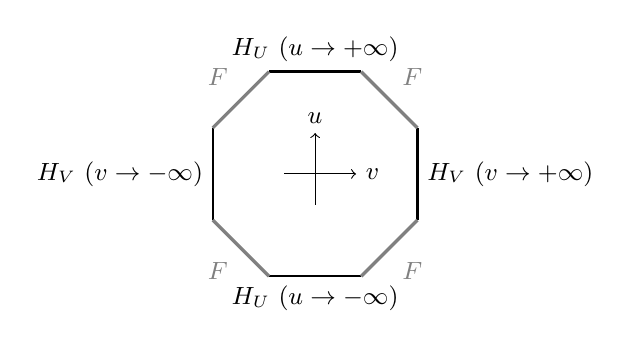
\begin{tikzpicture}[scale=1.3]
  \draw[thick] (-1,-0.45)--(-1,0.45) (1,-0.45)--(1,0.45)
               (-0.45,-1)--(0.45,-1) (-0.45,1)--(0.45,1);
  \draw[very thick,gray] (-1,0.45)--(-0.45,1) (0.45,1)--(1,0.45)
               (1,-0.45)--(0.45,-1) (-0.45,-1)--(-1,-0.45);
  \node[right] at (1,0) {\small $H_V$ ($v\to+\infty$)};
  \node[left] at (-1,0) {\small $H_V$ ($v\to-\infty$)};
  \node[above] at (0,1) {\small $H_U$ ($u\to+\infty$)};
  \node[below] at (0,-1) {\small $H_U$ ($u\to-\infty$)};
  \node[gray] at (0.95,0.95) {\small $F$};
  \node[gray] at (-0.95,0.95) {\small $F$};
  \node[gray] at (0.95,-0.95) {\small $F$};
  \node[gray] at (-0.95,-0.95) {\small $F$};
  \draw[->] (-0.3,0)--(0.4,0) node[right]{\small $v$};
  \draw[->] (0,-0.3)--(0,0.4) node[above]{\small $u$};
\end{tikzpicture}
\end{center}
Blowing down the four grey edges gives the square $\RC V\times\RC U$; blowing down the
four black edges to points gives the disc $\RC W$.

%----------------------------------------------------------------------
\subsection*{\Cref{distributions:ex:polar}}
Idea: by Hadamard's lemma a diffeomorphism fixing $0$ is $F(x)=G(x)x$ with $G(0)$
invertible, and then $F(r\omega)=rG(r\omega)\omega$ has a smooth polar form.
(This is the case of a point in $\R^n$ of \cref{blowup:thm:invariance}.)

Let $F\colon O\to O'$ be a diffeomorphism of open neighbourhoods of $0$ in $\R^n$ with
$F(0)=0$, and let $\epsilon_0>0$ with $B(0,\epsilon_0)\subset O$. For $|x|<\epsilon_0$,
\[
  F(x)=\int_0^1\frac{d}{dt}F(tx)\,dt=G(x)x,\qquad G(x)=\int_0^1DF(tx)\,dt,
\]
with $G$ smooth and $G(0)=DF(0)$ invertible. Choose $\epsilon\le\epsilon_0$ with $G(x)$
invertible for $|x|<\epsilon$. For $(r,\omega)\in(-\epsilon,\epsilon)\times\Sphere^{n-1}$
we have $F(r\omega)=r\,G(r\omega)\omega$ and $G(r\omega)\omega\neq0$. Define
\[
  \tilde F(r,\omega)=\Big(r\,|G(r\omega)\omega|,\ \frac{G(r\omega)\omega}{|G(r\omega)\omega|}\Big),
\]
which is smooth on $[0,\epsilon)\times\Sphere^{n-1}$ (indeed on $(-\epsilon,\epsilon)\times\Sphere^{n-1}$),
maps $\{r=0\}$ to $\{r=0\}$ and $\{r>0\}$ to $\{r>0\}$, and satisfies
$\tilde F(r,\omega)=(|F(r\omega)|,F(r\omega)/|F(r\omega)|)$ for $r>0$: it is $F$ written
in polar coordinates. On the boundary, $\tilde F(0,\omega)=(0,L\omega/|L\omega|)$ with
$L=DF(0)$, which is the action of $L$ on the sphere at infinity in
\cref{distributions:prop:affine}; for $F=L$ linear, $\tilde F(r,\omega)=(r|L\omega|,L\omega/|L\omega|)$
is exactly the linear case of the hint.

The same construction for $F^{-1}$ gives $\widetilde{F^{-1}}$, smooth on
$[0,\epsilon')\times\Sphere^{n-1}$. For $r>0$ small, polar coordinates are a
diffeomorphism onto a punctured ball, so $\widetilde{F^{-1}}\circ\tilde F=\Id$ and
$\tilde F\circ\widetilde{F^{-1}}=\Id$ where $r>0$ and both sides are defined; by
continuity these identities hold at $r=0$ as well. Choose $\delta>0$ so small that
$\widetilde{F^{-1}}$ maps $[0,\delta)\times\Sphere^{n-1}$ into $[0,\epsilon)\times\Sphere^{n-1}$
(possible since $\widetilde{F^{-1}}(r,\omega)$ has first component
$\le r\sup|G_{F^{-1}}|$). Then $\tilde F$ is a diffeomorphism from the open neighbourhood
$\tilde F^{-1}([0,\delta)\times\Sphere^{n-1})$ of $\{0\}\times\Sphere^{n-1}$ onto
$[0,\delta)\times\Sphere^{n-1}$, with inverse $\widetilde{F^{-1}}$. This is the asserted
diffeomorphism.

\emph{The blow-up of a point is well defined.} Let $(X,\beta)$ be a blow-up of $M$ at $p$
as defined in \cref{distributions:sec:other}, using local coordinates $x$ centred at $p$
in which polar coordinates $(r,\omega)\mapsto r\omega$ lift to a diffeomorphism $\kappa$
of a neighbourhood of $\pa X$ onto $[0,\epsilon)\times\Sphere^{n-1}$. (i) If $x'=F(x)$ is
another such coordinate system, then the polar coordinates of $x'$ are $\tilde F\circ\kappa$
near $\pa X$, again a diffeomorphism onto some $[0,\delta)\times\Sphere^{n-1}$. So the
condition in the definition does not depend on the coordinates. (ii) If $(X',\beta')$
is another blow-up of $M$ at $p$, the map $\beta'^{-1}\circ\beta\colon X\setminus\pa X\to
X'\setminus\pa X'$ is a diffeomorphism. Near the boundary, in the polar coordinates
of the two coordinate systems, it is $\tilde F$ (the identity if the same coordinates
are used), which extends smoothly with smooth inverse up to $r=0$. Hence
$\beta'^{-1}\circ\beta$ extends to a diffeomorphism $X\to X'$ commuting with the maps to
$M$. (iii) A blow-up exists: glue $M\setminus\{p\}$ and $[0,\epsilon)\times\Sphere^{n-1}$
along $(0,\epsilon)\times\Sphere^{n-1}\cong\{0<|x|<\epsilon\}$ by polar coordinates.
Thus $[M,\{p\}]$ is well defined up to unique diffeomorphism over $M$.
